\documentclass[a4paper, openany]{memoir}

\usepackage[utf8]{inputenc}
\usepackage[T1]{fontenc} 
\usepackage[english]{babel}
\usepackage{amsmath}
\usepackage{amssymb}

\usepackage{booktabs}
\usepackage{fancyhdr}
\usepackage{float}
\usepackage{indentfirst}
\usepackage{graphicx}
\usepackage[linewidth=1pt]{mdframed}
\usepackage{multicol}
\usepackage{fancyvrb}

\pagestyle{fancy}
\fancyhf{}
\fancyhead[LE]{\leftmark}
\fancyhead[RO]{\rightmark}
\fancyhead[RE, LO]{PSD}
\fancyfoot[LE, RO]{\thepage}
\fancyfoot[RE, LO]{Pete Gautam}

\renewcommand{\headrulewidth}{1.5pt}

\chapterstyle{thatcher}
\setcounter{chapter}{9}

\begin{document}

\chapter{Static Analysis}
Static analysis is a measurement that is applied to the source code or compiled application code of a system before execution. For example, we might count the number of import statements in a class file to give a measure of how coupled the class file is to other classes in the application.

Dynamic measurement is applied during execution itself. For example, the amount of time an application thread spends inside a class method or object can provide information about the amount of functionality provided by different parts of the application. Dynamic measurement is dependent on the specification of appropriate test scenarios in which we evaluate a design or ensure that the evaluation is realistic.

Confusingly, some measurements with the same name can be taken both statically and dynamically. For example, the number of method calls from one class to another can be measured statistically. This is done by counting the number of unique contexts in which a method is referenced from one class to another. It can also be done dynamically. We do this by counting all the invocations of a method that occur in the program execution. 

Although they are called the same, the two measures are giving us different data. Dynamically, the test indicates where performance optimisations might have the best benefit. On the other hand, statically, the test tells us whether a change to the code can be brittle.

Static analysis is an important tool in software engineering lifecycle. The static analysis tooling can detect a wide variety of potential defects. Tools are often used within the build pipeline, for which there are many use cases. 

A developer might use a static analysis tool to check changes on a branch before submission for code review. Continuous integration pipeline can also be configured to block merge requests that fail static analysis checks. This helps prevent defects entering the mainline of the software development project. 

Static analysis also optimises the code review process by ensuring that developers fix automatically detectable problems. It can also assist reviewers in assessing the proposed changes. It provides measurements of code that can help focus the attention.

The image below shows the spectrum of automated checks that can be performed on a source codebase.
\begin{figure}[H]
    \centering
    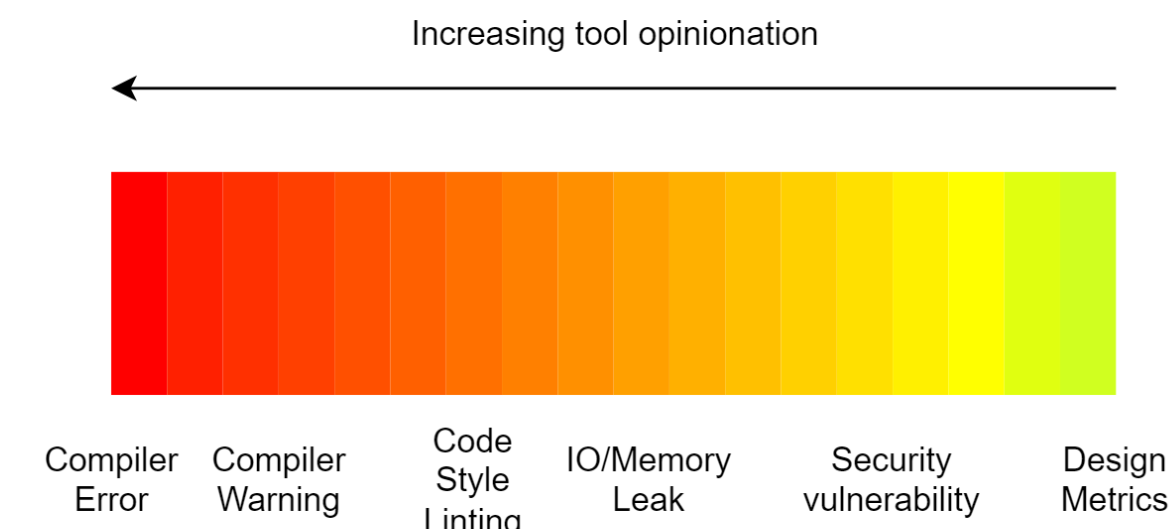
\includegraphics[scale=0.3]{src/10.1 opinionation.PNG}
\end{figure}
\noindent Opinionation increases as we go to the left. The opinionation of a tool increases as we can be more certain that there is a right way to do things. In some cases, this forces the developer to follow this approach.

The most obvious case is compiler/interpreter syntax errors. If the program cannot be understood by the compiler, then no binary will be produced. So, the program cannot be executed. At the other end of the spectrum, design metrics extracted from using static analysis tools need careful interpretation. They are often most useful for performing code reviews.

Static analysis fits in the middle. Warnings from static analysis tools can be compiler warnings and also design metrics at the other extreme. The design metrics do not have to be fixed for a program to be executed. But, doing so is likely to improve code quality and enhance long term maintainability.

In some ways, code reviews are also at the far right. If they are done well, code reviews should focus on high-level considerations informed by design metrics. These are meant to be more subjective by nature.

A key concept in readability is the notion of self-documenting code. Code is self-documenting if it doesn't require source code comments in order for it to be understood by another developer.

A significant benefit in self-documenting code is that it no longer becomes necessary to maintain a copy of the explanation of how the code works. A developer can simply look at the code itself and understand it.

\section{Code style standards}
To encourage the adoption of good standards in code style, a number of style guides exist. These are available for most languages. For example, there are official/community language guides for Python (the PEP8 standard), and vendor-driven styles for some languages, e.g. Eclipse for Java. 

The style guides are often written in a way that can be applied systematically. This has led to many linting tools that are available to check automatically whether code compiles with particular standards.

Code style standards cover a wide variety of issues. Some are listed below.
\begin{itemize}
    \item The maximum length of characters in a line of code. It is typically recommended to be 80 or 120 characters.
    
    \item Identifier naming conventions. There is a general move for readable code for literate variable name, i.e. \texttt{last\_commit\_file\_head} not \texttt{f\_hand}.
    
    \item Use of whitespace, both horizontal and vertical.
    
    \item Control structure usage. Some control structures become deprecated in a language over time, even though they are still permitted by the compiler.
    
    \item Use of parentheses. These can explicitly show the order of operations even though they might not be necessary.
    
    \item Redundant code, such as variables/functions declared that are never referenced.
    
    \item Implicit usage patterns, e.g. \texttt{isinstance(x, int)} instead of \texttt{type(x) == int}.
    
    \item Spelling. It is a good practice to avoid spelling mistakes in identifier names.
\end{itemize}

There are many linting tools available for a variety of different programming languages, e.g.
\begin{itemize}
    \item $\langle$X$\rangle$ Lint for most programming languages, PyLint.
    \item SonarQube for many languages.
    \item CheckStyle and FindBugs for Java.
\end{itemize}
Some modern compilers have linting built in as part of their warning and checks for code.

\section{Bug Detection}
As well as detecting poor style, many static analysis tools can detect usage patterns that are likely to indicate actual defects or bugs, such as:
\begin{itemize}
    \item property methods that can return null, e.g. in Python,
    \item access of null object parameters, e.g. variables that have not been initialised,
    \item inconsistent return statements in a method/function, e.g. there might be some blocks with explicit return statements and others in the same function that do not have a return statement,
    \item overloaded method names, and
    \item redefined/reassigned variables and parameters, which may indicate confused usage of the purpose of a parameter.
\end{itemize}

Static analysis tools can also be useful in detecting patterns of usage that might indicate a security vulnerability. For example, consider the following code.
\begin{verbatim}
Statement statement = conn.createStatement();
ResultSet resultSet = statement.executeQuery(
  "SELECT * FROM User WHERE User = `"+ user + "' AND password 
  = `" + password + "'");
\end{verbatim}
This is not the secure way of executing the query. If the user inputs the password to be the value \texttt{' OR TRUE OR password=`}. The code will always return the user object, so the attacker can easily bypass the authentication system.

Not only can static analysis tools automatically detect the vulnerability, they can also recommend a fix pattern. In the case of the code above, the recommended fix by static analysis is the following.
\begin{verbatim}
PreparedStatement preparedStatement =
  connection.prepareStatement("SELECT * FROM User WHERE User = ? 
  AND password = ?");
preparedStatement.setString(1, username);
preparedStatement.setString(2, password);
preparedStatement.executeQuery();
\end{verbatim}

Similarly, static analysis tools can detect poor usage patterns for I/O and memory management. For example, consider the following code.
\begin{verbatim}
try{
    FileInputStream fis = new FileInputStream("README.md");
    fis.read();
    //...
catch(IOException ioe){
    ioe.printStackTrace();
}
\end{verbatim}
If an exception occurs, the error gets printed. The file input stream is not explicitly closed by the developer in this branch. The recommended fix in this case is the following.
\begin{verbatim}
FileInputStream fis = null;
try{
    fis = new FileInputStream("README.md");
    fis.read();
    //...
catch(IOException ioe){
    ioe.printStackTrace();
} finally {
    if (fis != null){
        try{
            fis.close();
        } catch (IOException ioe){
            //handle exception
        }
    }
}
\end{verbatim}
The finally block closes the file no matter if an exception is thrown.

\section{Measuring Designs}
We can use static analysis tools to take measurements of software design. Some of these are listed below.
\begin{itemize}
    \item Cyclomatic complexity is useful for providing information about readability of code. The complex measures the complexity of paths through a function. It is measured by taking the number of edges (transitions between statements), and subtracting the number of nodes (the statements), and adding doubling the number of terminals (the exit points). That is,
    \[\text{complexity} = \text{edges} - \text{nodes} + \text{terminals} \cdot 2.\]
    For example, consider the following code.
    \begin{verbatim}
public static void printEvens(){
    for (int i = 0; i < 100; i++)
        if (i % 2 == 0)
            System.out.println(i);
}
    \end{verbatim}
    The cyclomatic graph for this code is given below.
    \begin{figure}[H]
        \centering
        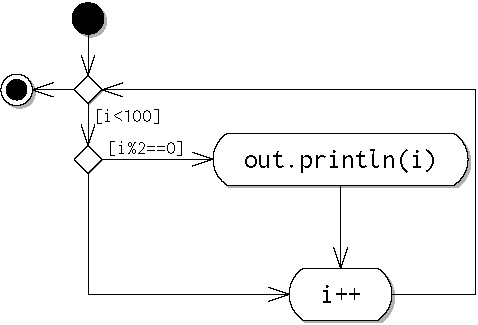
\includegraphics{src/10.2 cyclomatic flowchart.png}
    \end{figure}
    \noindent So, the complexity of the function is
    \[7 - 5 + 1 \cdot 2 = 4.\]
    It is recommended that the cyclomatic complexity for a function is less than 10.
    
    \item Nested scope depth is used to count nesting within a function. Consider the code below.
\begin{verbatim}
for (int i = 0; i < dimension; i++)
    for (int j = 0; j < dimension; j++)
        for (int k = 0; k < dimension; k++)
            for (int l = 0; l < dimension; l++)
                for (int m = 0; m < dimension; m++)
                    for (int n = 0; n < dimension; n++){
                        String message = "hello world " + 
                            "[%d,%d,%d,%d,%d,%d]";
                        System.out.println(
                            format(message,i,j,k,l,m,n));
                    }
\end{verbatim}
    The method has a highly nested structure. Such structures are difficult to maintain and read. Variables declared higher up in the scope are within scope much lower down and so can be altered and changed there. Cyclomatic complexity does not account for high nesting depth. An alternative metric we can use is nested scope depth. We count the total depth of steps of the blocks within each control structure. In this case, it is 6.
\end{itemize}

Another very useful measure for understanding designs is the rate of copuling between modules. There are a number of raw measures that can be used to calculate coupling between 2 modules. In particular, we can measure the following.
\begin{itemize}
    \item The number of method calls and variable accesses from one module to another.
    \item The number of import statements into a module.
    \item The number of type usages, e.g. the number of different types that are used in the module.
    \item The number of inheritance relations (above or below a class hierarchy).
\end{itemize}

Measurements can be taken in a variety of scopes. We might measure coupling at the scope of a single method, i.e. how coupled a single method is to another. Equally, we can measure coupling at class, module, package or application level.

Raw metrics can be gathered across different scope boundaries as well within scope boundaries. This provides additional insight. For example, we might want to calculate method calls between classes in different packages. This might be more significant form of coupling than method calls between classes in some packages.

\subsection{Fan in and Fan out complexity}
We can use raw measurements of coupling to calculate more sophisticated metrics. Fan in complexity describes the number of inbound references to a class/module from other modules. It is also called afferent coupling. It describes the number of classes that know about the class in consideration. Fan in complexity is useful for more precisely identifying the number of classes that have to be changed if the original class is changed.

Fan out complexity denotes the number of outbound references from a class to another. Fan out complexity is also called efferent coupling. It is a calculation of all the other classes that a class refers to. Fan out complexity is useful for determining how often a class may need to change because of the large number of classes it depends on.

\subsection{Inheritance depth and width}
Coupling can also be used to understand design considerations within an inheritance hierarchy. We might want to consider: depth and width of an inheritance hierarchy.
\begin{itemize}
    \item A very tall inheritance hierarchy (a hierarchy with high depth) may be problematic. It may indicate an over-abstraction. Moreover, the deeper the hierarchy becomes, the greater the potential for children and the harder it is to charge top-level class in hierarchy.
    
    \item A class with many children within an inheritance hierarchy may indicate the opportunity for introduction of intermediate abstractions. It may be because subsets of the children within the hierarchy actually have commonalities within themselves that may benefit from an intermediate abstraction being introduced. This reduces the amount of duplicate code in hierarchy.
\end{itemize}
Detection of bad smells in refactoring can be done using static analysis tools.

In summary, static analysis tools are an effective means of automatically detecting bugs and poor style. These can be estimated prior to the code review as part of a continuous integration pipeline.



\end{document}